In this section we break down the implementation of the system into its core components, following the methodology and requirements outlined in the previous sections. The full implementation can be found in the \ref{Appendix} appendix.

The resulting system consists of two main components. The \textbf{APR core} which holds the core logic for the repair process. The second component is the \textbf{Continuous Integration Pipeline} which integrates the core logic within a GitHub repository. It serves as the entry point and orchestrates the execution of the APR core based on configured triggers events of the repository.

\section{System Components}
%TODO ask ZHANG -> is this necessary and if components should be subsections
The implementation of the main components will be described in detail in the following section. The complete code implementation can be on GitHub listed in Appendix~\ref{Appendix}

\textbf{APR Core:}

% agent architectures produce good results epically paired with containerized environments. \cite{puvvadiCodingAgentsComprehensive2025}

The APR core contains the main bug fixing logic written in Python\footnote{todo ask ZHANG do i need this}. Embedding it into a Docker Image \footnote{link to docker} makes it easy to deploy, portable and small in memory. In order to use the APR core the following data needs to passed to the container:

\renewcommand{\arraystretch}{1.5} % Set row spacing to 1.5
\begin{longtable}{@{\extracolsep{\fill}} p{3.5cm} | p{7cm} | p{4cm}  @{}}
    \caption{Container Inputs} \label{tab:container-inputs}                                     \\

    \toprule
    \textbf{Name}      & \textbf{Description}                            & \textbf{Type}        \\
    \midrule
    \endfirsthead

    \bottomrule
    \endfoot
    Source Code        & Git repository where APR fix bugs               & Docker volume mount
    \\ \hline
    GITHUB\_TOKEN      & Token for GitHub API authentication             & Environment variable \\
    \hline
    LLM\_API\_KEY      & API key for the LLM provider                    & Environment variable \\
    \hline
    ISSUE\_TO\_PROCESS & The issue to process in JSON format             & Environment variable \\
    \hline
    GITHUB\_REPO       & GitHub repository for fetching and writing data & Environment variable \\
    \hline
\end{longtable}

With this environment set the APR core iterates over all issues which are fetched from the (ISSUE\_TO\_PROCESS) environment variable. For each issue the main APR logic is executed. This logic is a predefined flow which is makes use of multiple stages and tools.

At first a clean workspace and the issue repair context is set up. The context acts as the main data structure for the issue repair process and is used at every step. \ref{lst:context-json} shows what the context looks like when initialized.

\begin{lstlisting}[caption={Context JSON}, label={lst:context-json}]  
    context = {
        "bug": issue,
        "config": config,
        "state": {
            "current_stage": None,
            "current_attempt": 0,
            "branch": None,
            "repair_successful": False,
        },
        "files": {
            "source_files": [],
            "fixed_files": [],
            "diff_file": None,
            "log_dir": str(log_dir),
        },
        "stages": {},
        "attempts": [],
        "metrics": {
            "github_run_id": os.getenv("GITHUB_RUN_ID"),
            "script_execution_time": 0.0,
            "execution_repair_stages" : {},
            "tokens": {}
        },
    }
\end{lstlisting}

The context is used by a stage to perform a specific task in the bug fixing process and gets returns with the added context. The cores' stages are Localize, Fix, Build and Test.

The repair process starts with the localization stage. This stage tries to find the files needed from the codebase to fix the bug, using the configured LLM Model via the providers SDK\footnote{explain}. The localization prompt is build using the issue and a constructed hierarchy of the repositories file structure. The response is expected to return a list of files where the bug might be located. The localization system instruction and prompt are shown in \ref{lst:localization-prompt}.

\begin{lstlisting}[caption={Localization Prompt}, label={lst:localization-prompt}]
system_instruction = "You are a bug localization system. Look at the issue description and return ONLY the exact file paths that need to be modified."

prompt = f"""
    Given the following GitHub issue and repository structure, identify the file(s) that need to be modified to fix the issue.

    Issue #{issue['number']}: {issue['title']}
    Description: {issue.get('body', 'No description provided')}

    Repository files:
    {json.dumps(repo_files, indent=2)}

    Return a JSON array containing ONLY the paths of files that need to be modified to fix this issue.
    Example: ["path/to/file1.py", "path/to/file2.py"]
    """
\end{lstlisting}

With the localized files in the context the Fix stages comes next. Again this stage makes use of the configured LLM Model API to generate a fix for the issue in the localized files. The prompt for requesting the fix contains the issue details and file names with file content. The response is expected to contain a list of edits for each file. The LLM can also specify that no changes need to be made in a file. The generated response is then parsed and applied to the files in the workspace. Finally the context is updated with the new file content. Below is the system instruction and base prompt used for the Fix stage \ref{lst:repair-prompt}.

\begin{lstlisting}[caption={Repair Prompt}, label={lst:repair-prompt}]
system_instruction = "You are part of an automated bug-fixing system. Please return the complete, corrected raw source files for each file that needs changes, never use any markdown formatting. Follow the exact format requested."

base_prompt = f"""
    The following Python code files have a bug. Please fix the bug across all files as needed.

    {files_text}

    Please provide the complete, corrected source files. If a file doesn't need changes, you can indicate that.
    For each file that needs changes, provide the complete corrected file content.
    Format your response as:

    === File: [filepath] ===
    [complete file content or "NO CHANGES NEEDED"]

    === File: [filepath] ===
    [complete file content or "NO CHANGES NEEDED"]
    """
    
\end{lstlisting}

For validating the generated edits 2 stages are available; Build and Test. The Build stage is responsible for validating the syntax of the changes made in the Fix stage. It checks if the code can be built. For Python code this means checking if all syntax is valid and follows standardized code quality/maintenance rules \footnote{todo}. To archive this the code is first formatted using the Python formatter Black\footnote{todo} and secondly linted using flake8\footnote{todo}. This ensures properly formatted code and appends any warnings or errors to the context.

After validation the generated code is tested, if a test command is configured. The test stage runs the tests defined in the repository using the configured test command for each fixed file. In case tests fail, the context is updated with the error messages and the repair will jump back to the fix stage with a new attempt.

For a new attempt additional feedback is generated using the previous code and stage results with and attached to the prompt. When the maximum number of attempts is reached and the code does not pass testing an unsuccessful repair is reported to the issue by creating a comment using the Github API.

With successful validation and tests the issue is marked as a successfully repaired. The file changes are committed and pushed to the remote repository. A Pull Request is created to merge the issue branch in to the main branch. This Pull Request holds detailed file diffs and links the issue.

During execution the APR Core logs every action, which can be used for debugging makes the repair process more transparent. Furthermore it collects metrics such as the number of attempts, execution times, and token usage, which are essential for analyzing the effectiveness and performance of the APR system. A summary of the metrics is mentioned in \ref{section:evaluation}

The agent core is designed to be modular and extensible, allowing for future enhancements and additional stages or tools to be integrated as needed. It is also designed to be lightweight, ensuring that it can run efficiently within a CI/CD environment. Figure \ref{fig:apr-core} illustrates the functionalities and tools used in the APR Core.

\begin{figure}[H]
    \centering
    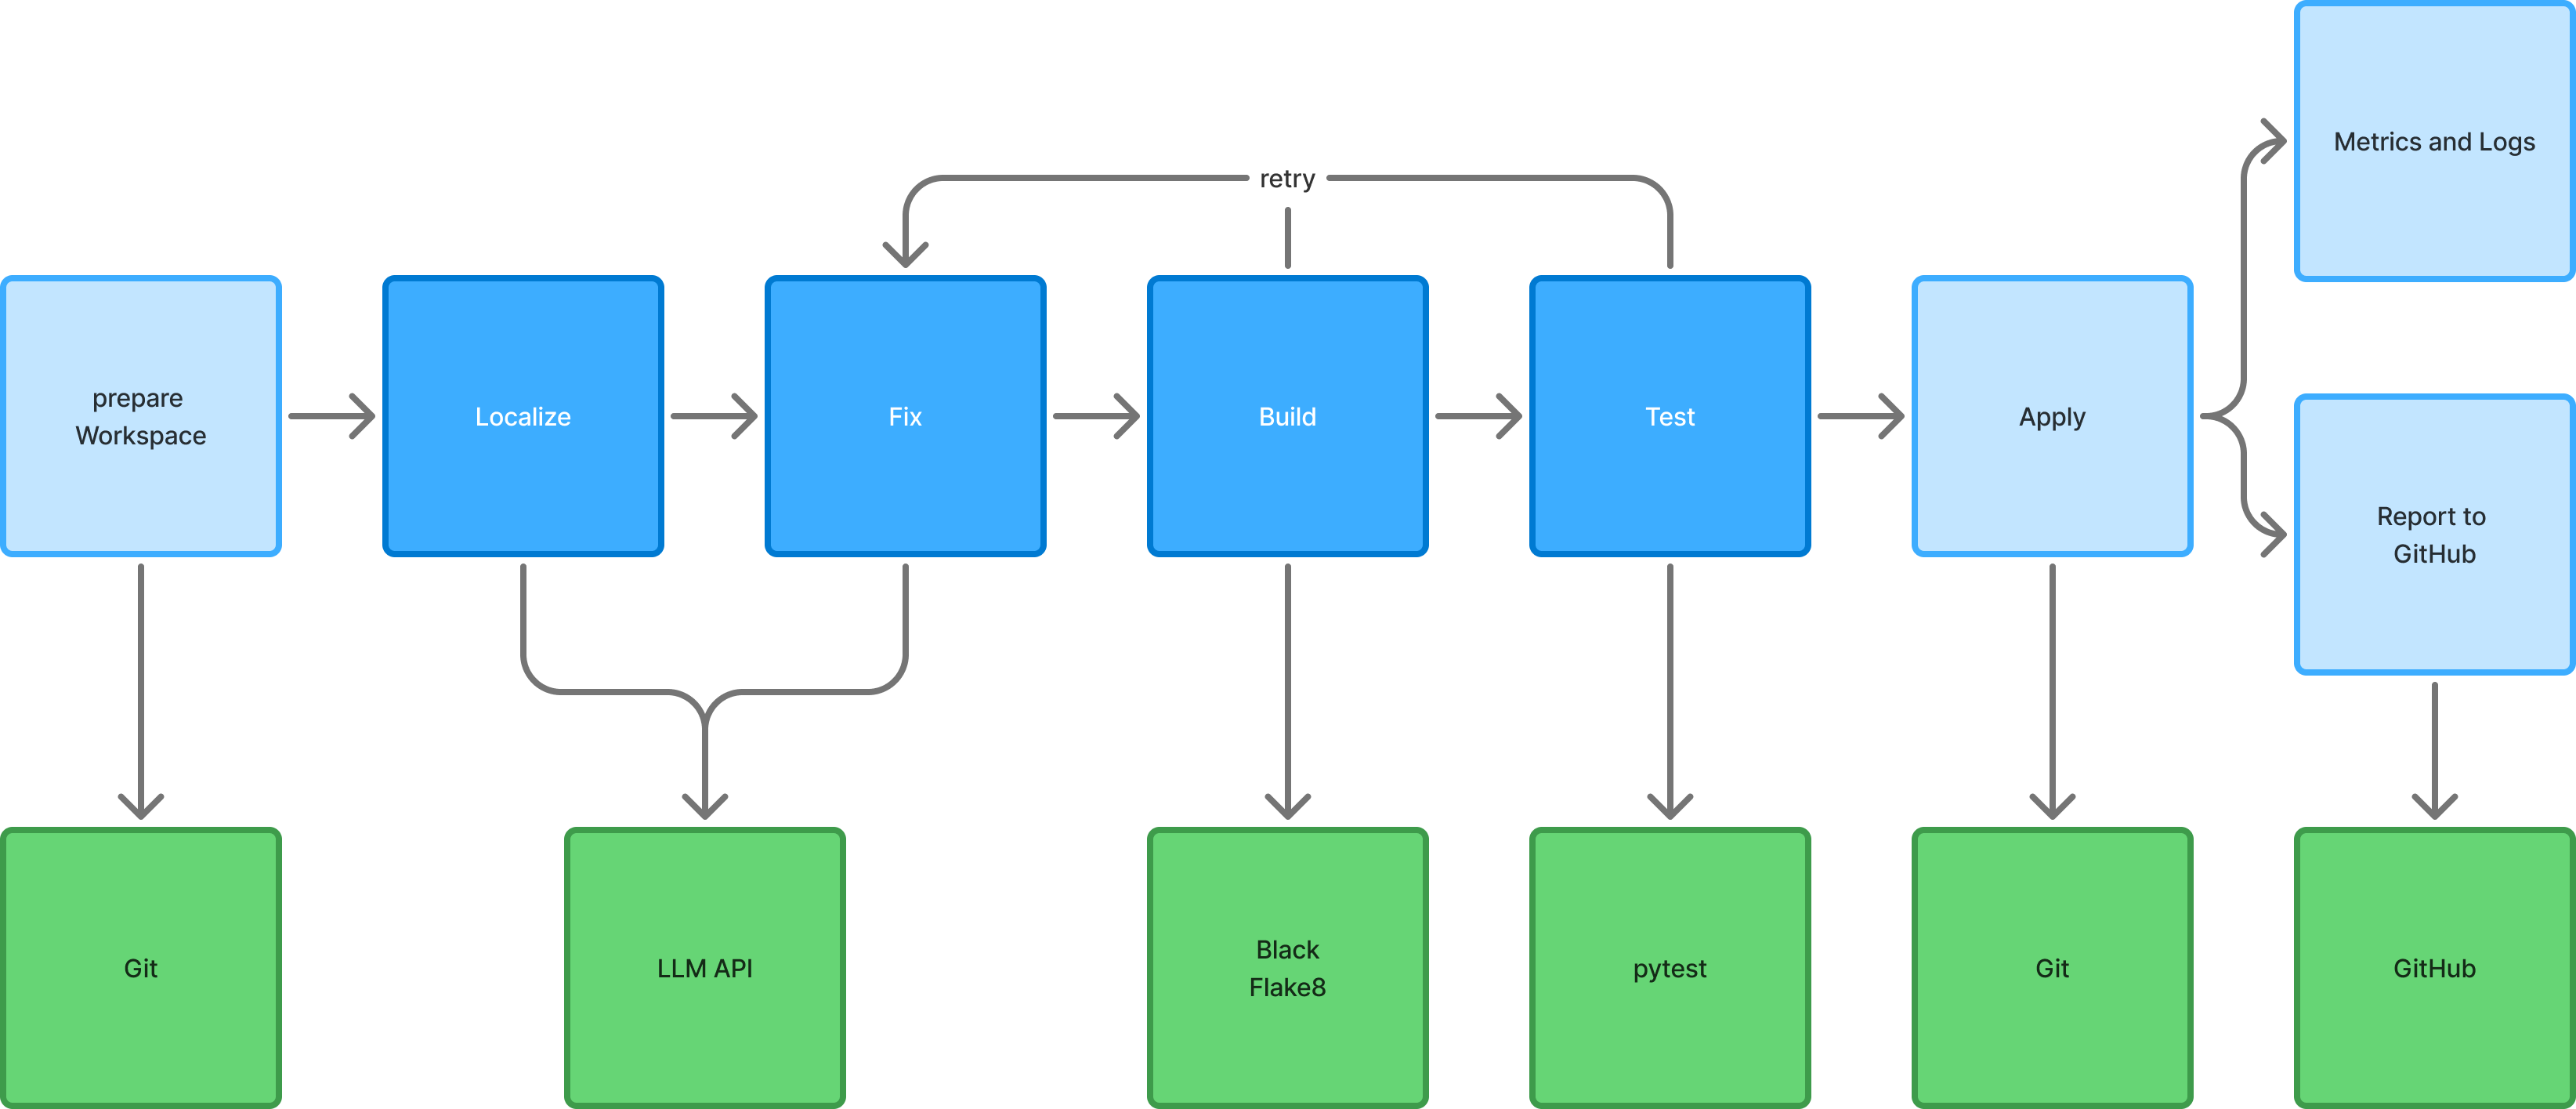
\includegraphics[width=1\textwidth]{images/flowcharts/apr-core.png}
    \caption{APR Core Logic}
    \label{fig:apr-core}
\end{figure}

\textbf{Continuous Integration Pipeline:}

A Github Action Workflow integrates the APR Core into the GitHub repository. The workflow is written in YAML\footnote{todo} according to the Github Action standard\footnote{link to GitHub}.
For this prototype we use linux x64 runners\footnote{default runner, sufficient for this purpose} provided and hosted by GitHub. This takes away the overhead of managing our own runners but comes at the cost of uncertain performance and availability. %\cite{}
The Workflow is made up of multiple triggers and jobs. Triggers are based on events\footnote{explain and link} from the GitHub repository and serve as the entry point for executing the jobs. Given the triggers the workflow can is executed two different ways:

\begin{itemize}
    \item Batch processing by fetching all issues with state for repair. This can be triggered by a manual dispatch (``workflow\_dispatch'') or scheduled execution (``cron'').
    \item Process a single issue from the event. The issue is passed from the (``issue\_labeld'') event when labeled with the configured labels or from (``issue\_comment'') when extra information is added issue in form of a comment.
\end{itemize}

The trigger event information gets passed as environment variables to the first job named ``gate''. This uses the data to determine if the issue should be processed or skipped using a python script (filter\_issues.py). This script needs be placed accessable for the workflow file. It checks labels of the issue and resolves its state to determine if the issue is relevant for the APR process. If no issues pass ``gate'' the job ``skipped'' is executed, which simply logs that no issues were found and exits the workflow run. In case issues  pass the ``gate'' the ``bugfix'' job is started. This job is responsible for executing the APR Core logic. It provides necessary prerequisites (see \ref{tab:container-inputs}) to start a container using the latest APR Core Docker Image which performs the the repair. These include checking out and mounting the code repository, setting environment variables, and providing the necessary permissions for the APR Core to edit repository content, create pull requests, and write issues on GitHub.

As the last step of ``bugfix'' is uploading the logs and metric files of the APR core as artifacts, which makes them available after the workflow run has completed.

Figure \ref{fig:ci} visualizes the workflow and its jobs.

\begin{figure}[H]
    \centering
    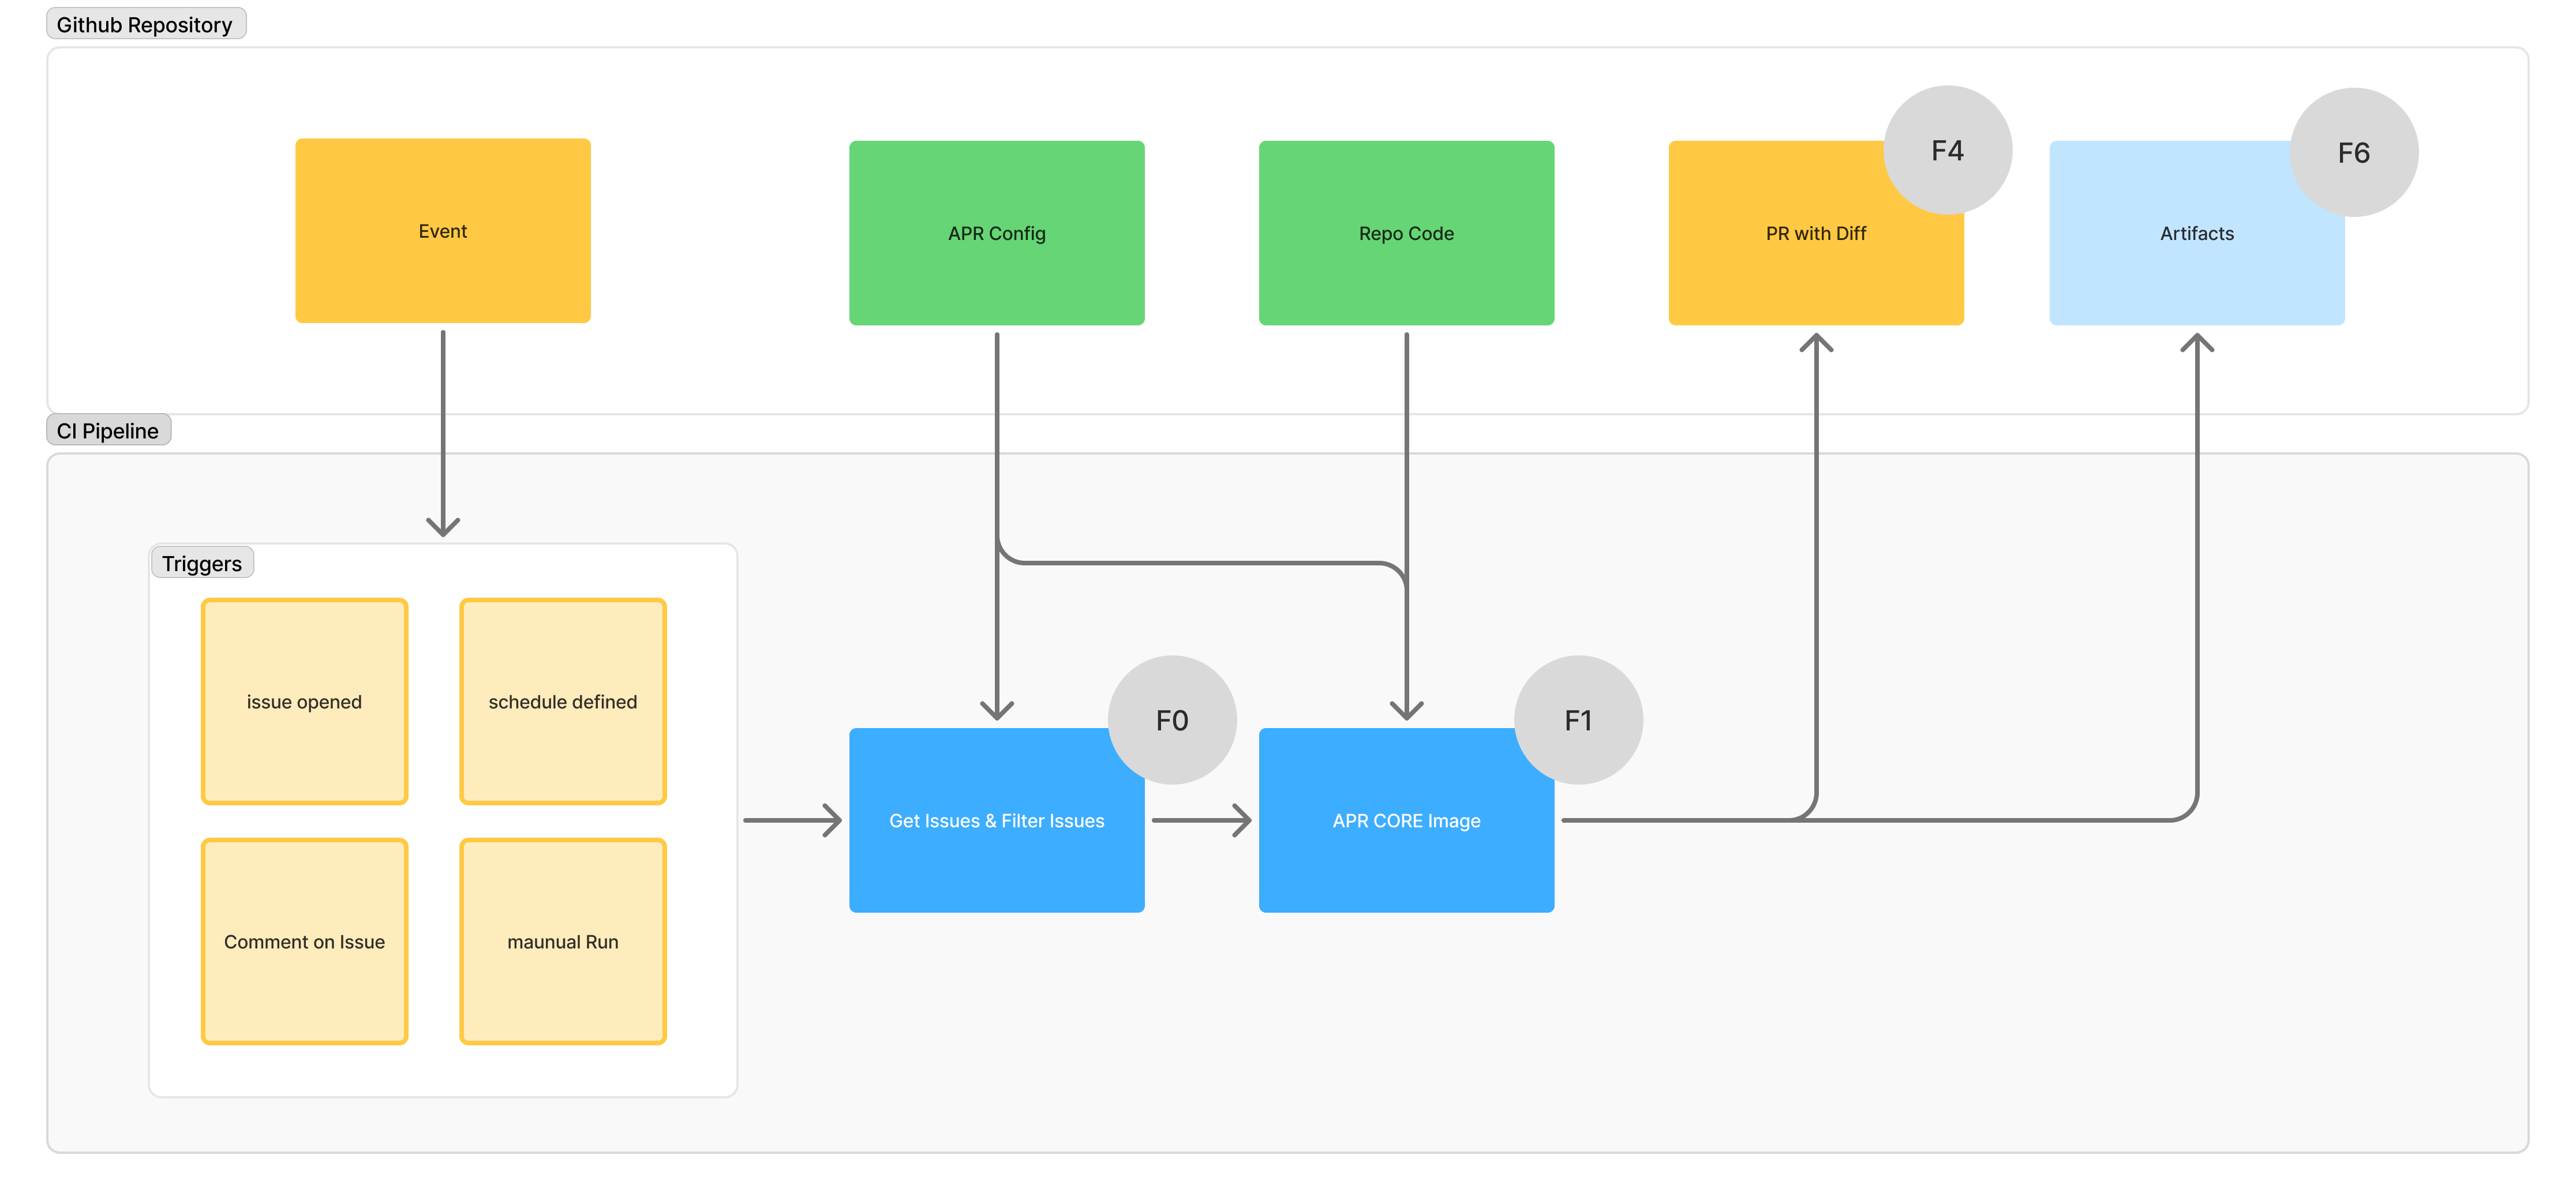
\includegraphics[width=1\textwidth]{images/flowcharts/ci.png}
    \caption{APR Core Logic}
    \label{fig:ci}
\end{figure}

For using this integration in a repository, the workflow file needs to be placed in the `.github/workflows` directory of the repository along with the `filter\_issues.py` in `.github/scripts`. With this in place an ``LLM\_API\_KEY'' needs to be set as a secret in the repository settings. This key is used by the APR Core to authenticate with the configured LLM provider API. Lastly GitHub Actions needs to be granted permissions to create pull requests and write issues in the repository. This is done by setting the workflow permissions in the repository settings under Actions -> General -> Workflow permissions.

\section{System Configuration}
%TODO add  collision avoidance
For making the system easily adjustable the APR Core and the CI Pipeline can be configured using a YAML configuration file. The configuration is optional when no configuration is in place the system will use default configuration. A custom configuration must be named ``bugfix.yml'' and must be placed at the root of the repository. This allows for easy customization of the system without changing the code itself. The configuration read by system components during execution. Table \ref{table:configuration} lists the available configuration fields with a  description.

\renewcommand{\arraystretch}{1.5}
\begin{longtable}{@{\extracolsep{\fill}} p{3.5cm} | p{11cm} @{}}
    \caption{Configuration Fields and Descriptions} \label{table:configuration}                                                         \\
    \toprule
    \textbf{Configuration Field} & \textbf{Description}                                                                                 \\
    \midrule
    \endfirsthead

    \bottomrule
    \endfoot

    to\_fix\_label               & The label used to identify issues that need fixing.                                                  \\ \hline
    submitted\_fix\_label        & The label applied to issues when a fix is submitted.                                                 \\ \hline
    failed\_fix\_label           & The label applied to issues when a fix fails.                                                        \\ \hline
    workdir                      & The working directory where the code resides, used for mounting in the Docker container.             \\ \hline
    test\_cmd                    & The command used to run tests on the codebase.                                                       \\ \hline
    branch\_prefix               & The prefix for branches created for bug fixes, allowing for easy identification of bug fix branches. \\ \hline
    main\_branch                 & The main branch of the repository where bug fix branches are based.                                  \\ \hline
    max\_issues                  & The maximum number of issues to process in a single run.                                             \\\hline
    max\_attempts                & The maximum number of attempts to fix an issue before giving up.                                     \\ \hline
    provider                     & The LLM provider used for generating fixes.                                                          \\ \hline
    model                        & The specific model from the LLM provider used for generating fixes.                                  \\
\end{longtable}



\section{Requirement Validation}

The following sections outline how each requirement was satisfied.

